\section{Response Length}

\begin{figure}[H]
    \centering
    % 如果是单栏排版，建议将宽度设为 \linewidth 或 0.9\linewidth
    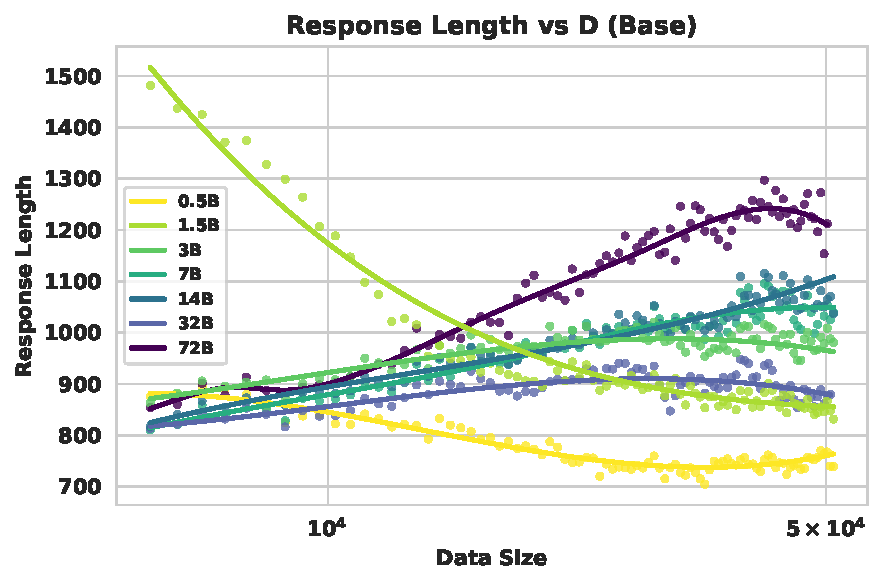
\includegraphics[width=\linewidth]{./figures/outputs/outputs/response_base_response_length_N_E_R.pdf}
    \caption{\tzl{Response length vs.\ Data size (Base models).}}
    \label{fig:limiting_plots_base}
\end{figure}

\begin{figure}[H]
    \centering
    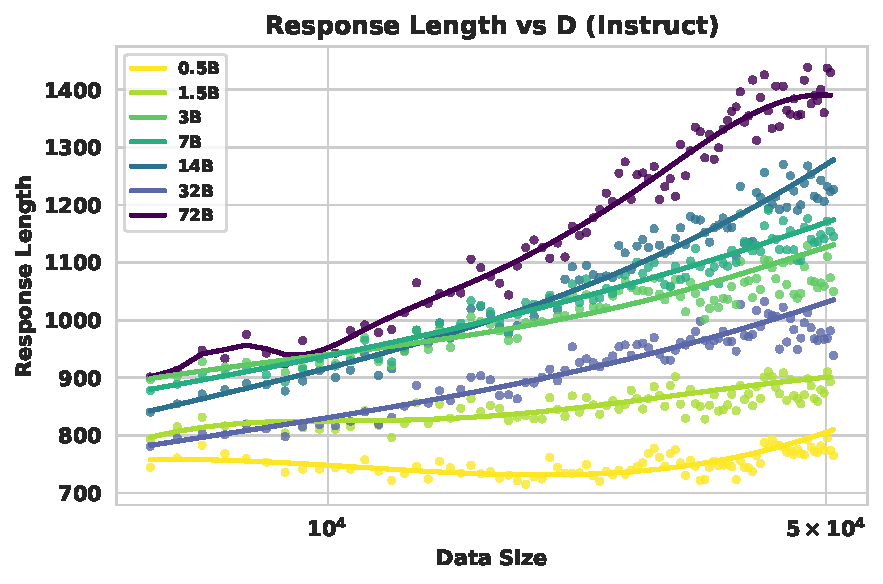
\includegraphics[width=\linewidth]{./figures/outputs/outputs/response_instruct_response_length_N_E_R.pdf}
    \caption{\tzl{Response length vs.\ Data size (Instruct models).}}
    \label{fig:limiting_plots_instruct}
\end{figure}



% \begin{figure}[H]
%     \centering
%     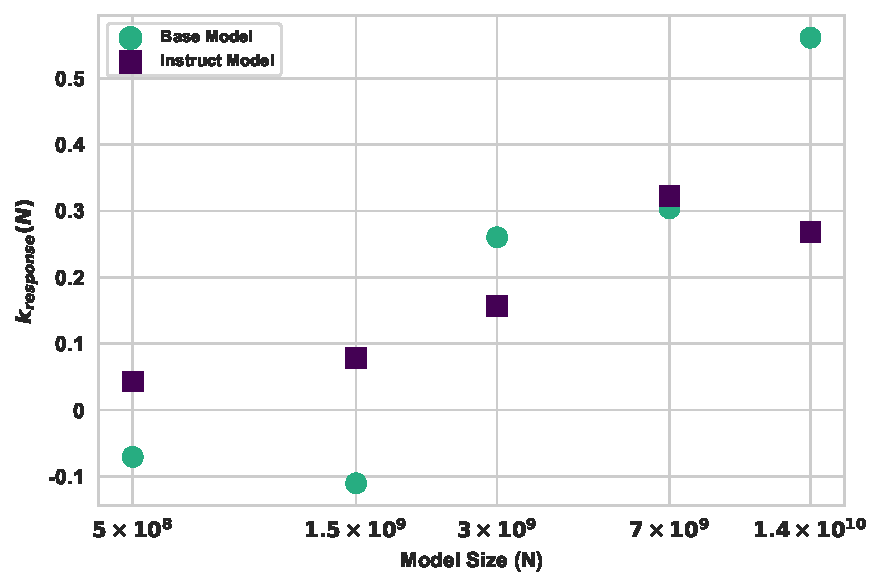
\includegraphics[width=0.48\textwidth]{./figures/response_length/base_vs_instruct_L-N-response_length_fitting_comparison_k.pdf}
%     % 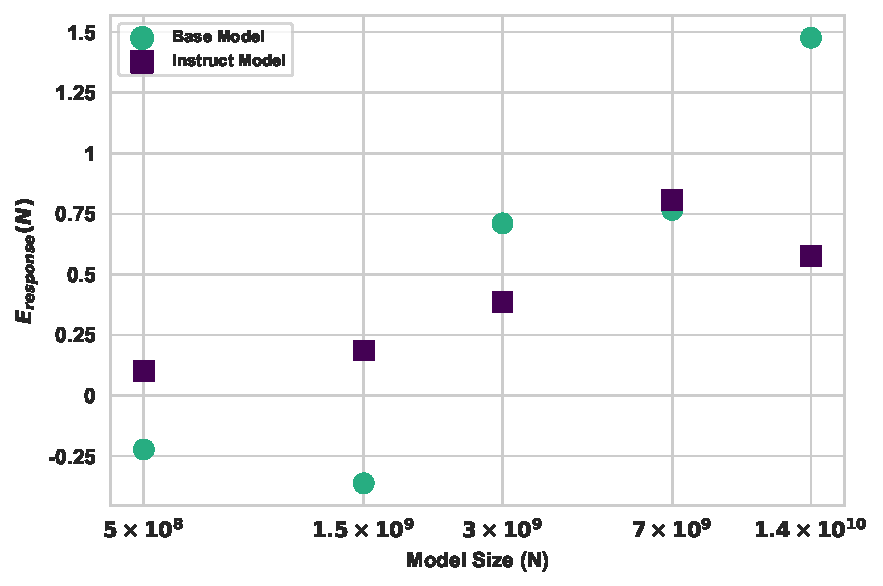
\includegraphics[width=0.48\textwidth]{./figures/response_length/base_vs_instruct_L-N-response_length_fitting_comparison_E0.pdf}
%     \caption{Fitted response length parameters vs. Model Size. Left: $k_\text{response}(N)$. Right: $E_\text{response}(N)$.}
%     \label{fig:limiting_plots_wholefitted}
% \end{figure}

% \begin{wrapfigure}{r}{0.45\textwidth}
%     \centering
%     \vspace{-1em} % 调整竖直位置，避免顶到段落
%     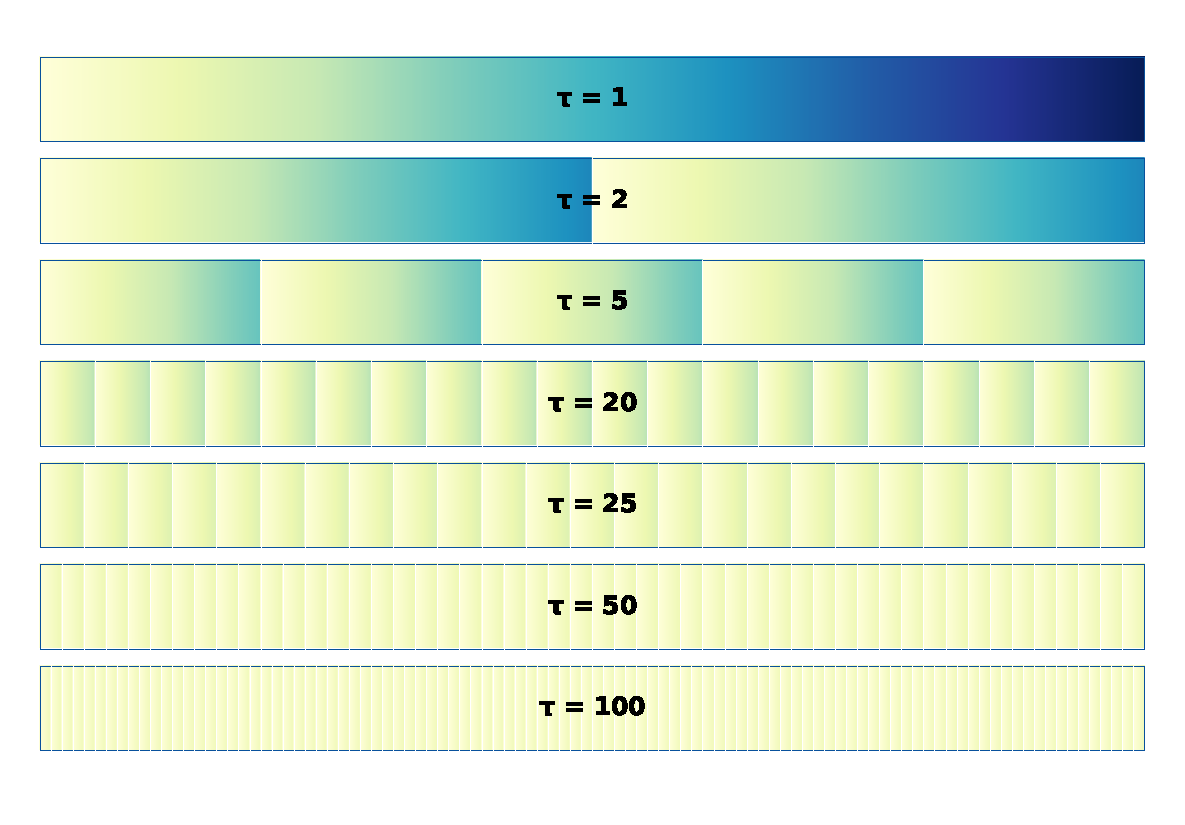
\includegraphics[width=0.95\linewidth]{./figures/datareuse/exp2_tau_rectangles.pdf}
%     \caption{Data Reuse Schema}
%     \label{fig:data_reuse_schematic}
% \end{wrapfigure}

% 1.  越大的模型response length span越大
% 2. 3B以上response 效率拐点
% 3. 3B以下response 效率反而略有降低，3B是可观测response效率最差model
% 4. 这里的k_response(N)趋势表示越大模型对于response的利用率越有效，对小模型来说增大response length对效果提升也没啥用，都是乱说